\chapter{Implementation}
\label{chap:Implementation}
This chapter will describe the implementation of the systems components. It will cover the description of the Microsoft Kinect, the robot's code and how the scheduling is done. 

\section{Microsoft Kinect}
\label{sec:Microsoft Kinect Implementation}

\section{Robot}
\label{sec:Robot}

\section{Scheduling}
\label{sec:Scheduling implementation}

\subsection{UPPAAL schedulability analysis}
\label{sec:UPPAAL schedulability}
As described in Appendix \ref{sec:i3UPPAAL model}, Dumpsty contains three tasks: PrA, PrB and PrC. These three tasks all have individual WCET, which is not calculated, but rather tested, since calculating these through assembly proved to be impossible due to unbound loops in libraries. After testing the individual task's WCET, the worst case found would be significantly faster than what is labelled in UPPAAL, since the probability of hitting the actual worst case is close to impossible with the amount of tests done. In the following bulletpoints, all three tasks tested WCET and the WCET used in UPPAAL for the specific task is expressed, which is the first step to verify the schedulability of Dumpsty's tasks.

\begin{itemize}
	\item PrA \tab Tested: 1067 microseconds \tab UPPAAL: 2 milliseconds
	\item PrB \tab Tested: 732  microseconds \tab UPPAAL: 1 milliseconds
	\item PrC \tab	Tested: 8469 microseconds \tab UPPAAL: 9 milliseconds
\end{itemize}

For convenience, and to simplify the analysis, all tasks contain the worst case runtime of all interrupts and interrupt handlers that might occur during the execution of the task. These interrupts are generated by the motor encoders when Dumpsty is moving.

Figure 5.1 depicts the automatas created in UPPAAL from two declared classes. The first class, task PrA, is the cyclic executive instance for the task PrA. The second class is simply a CPU which is the key needed to run the task. Every task can grab the CPU, but only one may hold it at any given time. The CPU is then released when the task is done executing, and another task can then proceed to run.

\begin{figure}[h]
	\centering
	\fbox{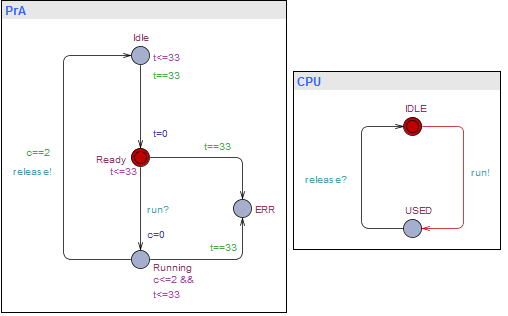
\includegraphics[scale=0.60]{billeder/UPPAALPr}}
	\caption{Automata in UPPAAL}
	\label{robot}
\end{figure}
